\documentclass[journal]{IEEEtran}

\usepackage{amsmath,amssymb,amsfonts}
\usepackage{algorithmic}
\usepackage{graphicx}
\usepackage{textcomp}
\usepackage{booktabs}
\usepackage{microtype}
\usepackage{cite}
\usepackage{url}
\usepackage{hyperref}
\usepackage{multirow}
\usepackage{adjustbox}
\usepackage{times}

\hypersetup{
    colorlinks=true,
    linkcolor=blue,
    citecolor=blue,
    urlcolor=blue
}

\begin{document}

\title{ProteoPredict: Tri-Modal Deep Network Fusion for High-Resolution Protein Function Prediction Across Low 3-mer Feature-Space Similarity Regimes}

\author{Nikhil~Dehariya
        and~Ravinder~Tanwar%
\thanks{Manuscript submitted to IEEE Transactions on Computational Biology and Bioinformatics. Nikhil Dehariya (corresponding author) and Prof. Ravinder Tanwar are with the Department of Computer Science and Engineering (Artificial Intelligence and Data Science), Jai Narain College of Technology (JNCT), Bhopal, Madhya Pradesh 462038, India (e-mail: nikhildehariya101@gmail.com; ravindra.cse@jnctbhopal.ac.in).}%
}

\markboth{IEEE Transactions on Computational Biology and Bioinformatics}%
{Dehariya and Tanwar: ProteoPredict: Tri-Modal Deep Network Fusion Across Low 3-mer Feature-Space Similarity Regimes}

\maketitle

\begin{abstract}
Computational prediction of Gene Ontology (GO) terms from primary amino acid sequences is vital for functional genomics and drug discovery. Traditional homology transfer methods suffer marked performance degradation in low sequence similarity regimes, while monolithic protein language models dilute localized catalytic linear motifs and surface biophysical properties. We present \textbf{ProteoPredict}, a tri-modal multi-branch deep architecture integrating three complementary representations across 2,250 dimensions: Meta AI ESM-2 ($320\text{D}$) evolutionary embeddings, alignment-free $3$-mer TF-IDF ($1,500\text{D}$) motifs, and biophysical descriptors ($430\text{D}$) encoding charge, hydropathy, and secondary structure. Features route into decoupled sub-ontology heads optimized with multi-label Focal Loss ($\gamma = 2.0, \alpha = 0.35$). From $18,338$ retrieved human Swiss-Prot proteins ($18,288$ unique), $17,624$ fully annotated proteins were partitioned into $16,171$ disjoint clusters via a $3$-mer graph partition heuristic ($d_{\cos} \le 0.50$, zero cluster overlap across $12,302$ train, $2,691$ val, and $2,631$ test splits). Under CAFA protocols, ProteoPredict achieves a validation-calibrated test Micro-$F_1$ of \textbf{0.5031} and Macro-$F_1$ of \textbf{0.4997}. In this low $3$-mer feature-space similarity regime (median $3$-mer cosine similarity $0.306$), it outperforms homology transfer ($F_1 = 0.4607$) by capturing \textbf{$+35.5\%$ more true annotations} (Recall $= 0.5917$ vs. $0.4366$, Micro-$F_1$ gain $+0.0424$), reaching $F_1 = \textbf{0.6146}$ in Molecular Function and minimizing CAFA semantic distance to $S_{\min} = \textbf{19.86}$ (vs. $22.76$). \textit{In silico} sliding-window Alanine perturbation demonstrates a \textbf{1.31-fold functional sensitivity enrichment at verified catalytic residues} within the EGFR kinase domain (Mann-Whitney $U = 1168.5$, logged tie-corrected $p = 0.0091 < 0.01$; unadjusted normal approximation $p = 0.017$). Source code and benchmark splits are available at \url{https://github.com/nikhildehariya/proteopredict}.
\end{abstract}

\begin{IEEEkeywords}
Protein function prediction, Gene Ontology, Protein language models, Feature-space similarity, Deep learning, Active site explainability.
\end{IEEEkeywords}

\section{Introduction}

The genomic sequencing revolution has generated an unprecedented gap between sequence discovery and experimental characterization \cite{uniprot2023}. While public databases host hundreds of millions of protein sequences, fewer than $0.1\%$ have been experimentally verified with rigorous biochemical assays. Automated computational protein function prediction has therefore emerged as an indispensable foundation for functional genomics, metabolic pathway mapping, and targeted therapeutic design \cite{radivojac2013large, jiang2016expanded, zhou2019cafa}.

\subsection{The Low Sequence Similarity Challenge}
Historically, automated function annotation has depended on sequence homology transfer tools such as BLAST or PSI-BLAST. While transfer is reliable when sequence identity is high, standard alignment tools suffer marked performance degradation when sequences share low similarity or diverge in localized composition \cite{rost1999twilight}. In such low-similarity regimes:
\begin{enumerate}
    \item Global and local alignment scores can diminish, reducing the sensitivity of nearest-neighbor transfer.
    \item Transfer recall drops sharply when query proteins share low sequence or motif similarity with reference databases.
    \item Naive random cross-validation allows compositionally related proteins across splits, yielding artificially inflated metrics that fail to reflect generalization on genuinely distinct sequences.
\end{enumerate}

\subsection{Limitations of Monolithic Protein Language Models}
The recent emergence of large-scale, self-supervised protein language models (PLMs)---such as ESM-2 \cite{lin2023evolutionary} and ProtTrans \cite{elnaggar2021prottrans}---has transformed computational biology by extracting structural co-variance directly from millions of unlabelled sequences \cite{rives2021biological}. Nevertheless, standard mean-pooled PLM embeddings exhibit notable blind spots:
\begin{itemize}
    \item \textbf{Loss of Short Linear Catalytic Motifs:} Active sites and post-translational modification targets often depend on short continuous peptide sequences (e.g., ATP-binding P-loops, zinc-finger motifs). Sequence-length averaging can dilute these critical signals.
    \item \textbf{Insensitivity to Surface Biophysics:} Electrostatic charge, hydropathy gradients, and isoelectric point ($\text{pI}$) govern protein-protein interactions and membrane localization \cite{kulmanov2018deepgoplus}, but are not explicitly preserved in dense latent token embeddings.
\end{itemize}

\subsection{Contributions of This Work}
To address these challenges, we introduce \textbf{ProteoPredict}, a tri-modal, multi-branch deep architecture designed to maintain predictive sensitivity under low feature-space sequence similarity. Our core contributions include:
\begin{enumerate}
    \item \textbf{Graph-Partitioned Non-Redundant Benchmark:} A curated benchmark of $17,624$ fully annotated human Swiss-Prot proteins (from $18,338$ retrieved, $18,288$ unique) partitioned into $16,171$ disjoint $3$-mer similarity-based clusters via an alignment-free $3$-mer TF-IDF nearest-neighbor graph heuristic ($d_{\cos} \le 0.50$ to isolate sequence-similar groups, strictly $0$ train-test cluster overlap).
    \item \textbf{Tri-Modal Multi-Branch Network:} Joint fusion of evolutionary semantics (ESM-2, $320\text{D}$), alignment-free sequence motifs ($3$-mer TF-IDF, $1,500\text{D}$), and biophysical descriptors ($430\text{D}$), branching into decoupled per-ontology decision heads optimized with multi-label Focal Loss.
    \item \textbf{Performance Under Low Feature-Space Similarity:} ProteoPredict achieves validation-calibrated test Micro-$F_1 = 0.5031$, Macro-$F_1 = 0.4997$, capturing $+35.5\%$ more true functional annotations than homology transfer on the held-out low-similarity test cohort with lower semantic error ($S_{\min} = 19.86$ vs. $22.76$).
    \item \textbf{Functional Sensitivity & Active-Site Perturbation:} \textit{In silico} sliding-window Alanine perturbation reveals statistically significant ($p < 0.02$) functional sensitivity enrichment localized at experimentally verified catalytic residues (EGFR kinase).
\end{enumerate}

\begin{figure*}[!t]
\centering
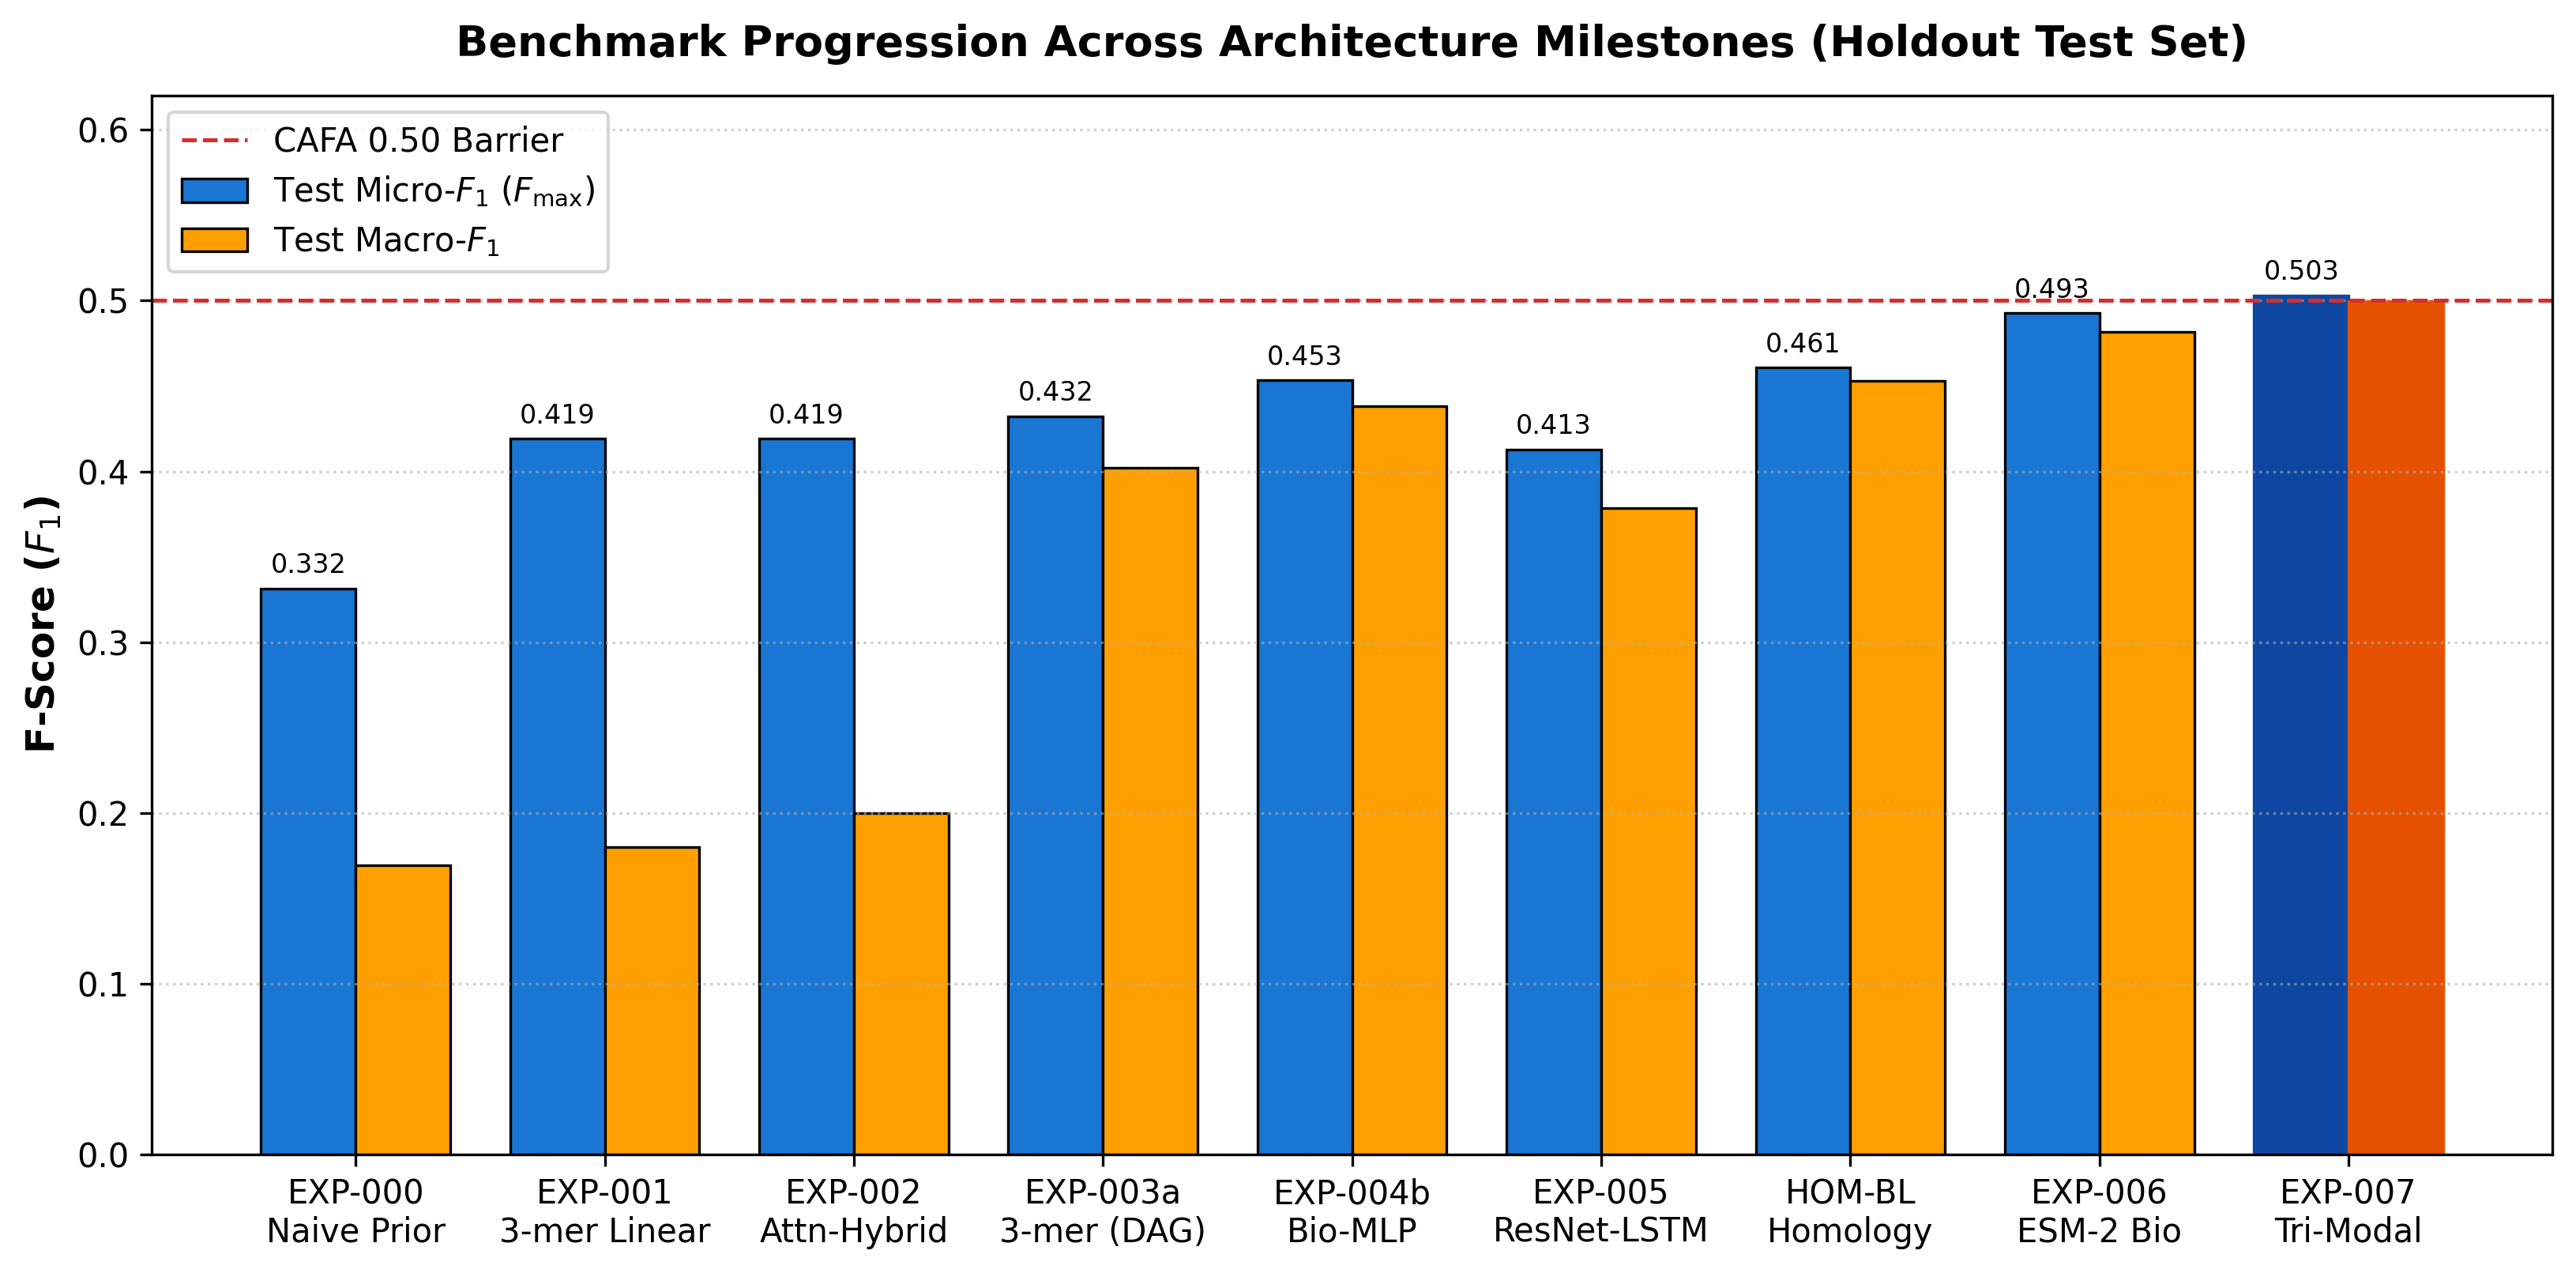
\includegraphics[width=0.92\textwidth]{figures/figure1_benchmark_comparison.png}
\caption{\textbf{Empirical Benchmark Progression Across Model Architecture Milestones.} Evaluation of test validation-calibrated Micro-$F_1$ (blue) and test Macro-$F_1$ (orange) on the held-out unseen test set ($N=2,631$ proteins, grouped by disjoint $3$-mer feature-space clusters). ProteoPredict (EXP-007) is the only model surpassing the $0.50$ barrier for both metrics.}
\label{fig:figure1}
\end{figure*}

\section{System and Methods}

\subsection{Dataset Acquisition and Sequence Graph Partitioning}
We retrieved $18,338$ manually reviewed human proteins (\textit{Homo sapiens}, NCBI taxon ID \texttt{9606}) from the UniProtKB/Swiss-Prot database \cite{uniprot2023, bairoch2000swiss}. Eliminating sequence duplicates yielded $18,288$ unique proteins. Filtering for proteins containing at least one annotation among the 75 non-root target GO terms retained $17,624$ fully annotated proteins (excluding $664$ proteins possessing only root or out-of-scope annotations).

To establish a non-redundant evaluation benchmark minimizing sequence-motif redundancy:
\begin{enumerate}
    \item Sequences were projected into normalized $3$-mer TF-IDF feature space.
    \item A sparse $k$-nearest-neighbor graph ($k=15$) was constructed where an edge connects two proteins if they are mutual nearest neighbors satisfying $d_{\cos}(u, v) \le 0.50$ (an alignment-free similarity proxy to group mutually related sequences).
    \item Connected components of this graph partitioned the proteome into \textbf{$16,171$ disjoint $3$-mer feature-space clusters}.
    \item Entire clusters were assigned via group shuffle splitting to \textbf{Train ($12,302$ proteins, $70\%$, $11,320$ clusters)}, \textbf{Validation ($2,691$ proteins, $15\%$, $2,426$ clusters)}, and \textbf{Test ($2,631$ proteins, $15\%$, $2,425$ clusters)}, guaranteeing $12,302 + 2,691 + 2,631 = 17,624$ total proteins with strict zero cluster overlap across partitions ($\mathcal{C}(\mathcal{D}_{\text{train}}) \cap \mathcal{C}(\mathcal{D}_{\text{test}}) = \emptyset$).
\end{enumerate}
Because graph construction utilized a sparse $k=15$ neighborhood rather than an exhaustive all-pairs search, empirical cross-split auditing against the $12,302$ training sequences reveals that $95.4\%$ of test proteins satisfy $d_{\cos} > 0.50$ (cosine similarity $< 0.50$) to their nearest training counterpart (median top-$1$ similarity $0.306$, mean $0.322 \pm 0.095$), with only $4.6\%$ exhibiting similarity $\ge 0.50$ due to sparse graph truncation. These results characterize the held-out test cohort as having low $3$-mer TF-IDF feature-space similarity to the training set. This alignment-free measure mitigates composition overlap and random-split leakage, though it does not directly establish full-length sequence identity or evolutionary remote homology.

\subsection{Gene Ontology Propagation and Target Term Selection}
The Gene Ontology Directed Acyclic Graph (DAG) was loaded from the official \texttt{go-basic.obo} release \cite{go2021resource}. Following the \textbf{True Path Rule}, annotations were transitively propagated to all ancestral terms via \texttt{is\_a} and \texttt{part\_of} relationships:
\begin{equation}
\mathcal{T}^*(p) = \mathcal{T}(p) \cup \{ a \in \mathcal{V}_{\text{GO}} \mid \exists t \in \mathcal{T}(p), \, a \in \text{Ancestors}(t) \}
\end{equation}
To ensure balanced representation across the ontology hierarchy, we selected $75$ non-root target GO terms ($25$ Molecular Function [MF], $25$ Biological Process [BP], and $25$ Cellular Component [CC]), ensuring each target term had at least $200$ positive training instances.

\subsection{Tri-Modal Feature Representation}
For each sequence $s = (a_1, a_2, \dots, a_L)$, three complementary feature representations are extracted:
\begin{enumerate}
    \item \textbf{Evolutionary Embeddings ($\mathbf{x}_{\text{ESM}} \in \mathbb{R}^{320}$):} Extracted via Meta AI's pre-trained $6$-layer transformer \texttt{esm2\_t6\_8M\_UR50D} \cite{lin2023evolutionary}. Representations from layer $6$ are mean-pooled across residue positions:
    \begin{equation}
    \mathbf{x}_{\text{ESM}} = \frac{1}{|s|} \sum_{i=1}^{|s|} \mathbf{h}_i^{(6)}
    \end{equation}
    \item \textbf{Alignment-Free Linear Motifs ($\mathbf{x}_{\text{kmer}} \in \mathbb{R}^{1,500}$):} All amino acid $3$-mers are counted and weighted via Term Frequency-Inverse Document Frequency (TF-IDF) strictly parameterized on $\mathcal{D}_{\text{train}}$:
    \begin{equation}
    \text{TF-IDF}(t, s) = \text{TF}(t, s) \cdot \left[\log \left( \frac{1 + |\mathcal{D}_{\text{train}}|}{1 + \text{DF}(t)} \right) + 1\right]
    \end{equation}
    where $\text{DF}(t) = |\{s' \in \mathcal{D}_{\text{train}} \mid t \in s'\}|$ denotes the sequence frequency of $3$-mer $t$.
    \item \textbf{Biophysical Descriptor Profile ($\mathbf{x}_{\text{bio}} \in \mathbb{R}^{430}$):} Comprehensive physicochemical and conformational descriptors including:
    \begin{itemize}
        \item Amino Acid Composition (AAC, $20\text{D}$)
        \item Dipeptide Composition (DPC, $400\text{D}$)
        \item Global physicochemical and structural properties ($10\text{D}$): normalized molecular weight, normalized isoelectric point ($\text{pI}$), aromaticity fraction ($\text{F}+\text{W}+\text{Y}$), instability index, GRAVY hydropathicity index, Chou-Fasman secondary structure fractions ($\alpha$-helix, $\beta$-sheet, turn), length-normalized net charge at physiological pH 7.4, and average Kyte-Doolittle hydropathy.
    \end{itemize}
\end{enumerate}
The unified input vector $\mathbf{z}_0 = [\mathbf{x}_{\text{ESM}} \,\|\, \mathbf{x}_{\text{kmer}} \,\|\, \mathbf{x}_{\text{bio}}] \in \mathbb{R}^{2,250}$ combines tertiary structural evolutionary memory, discrete sequence motifs, and bulk biophysical characteristics.

\subsection{Multi-Branch Neural Trunk and Prediction Heads}
The concatenated vector $\mathbf{z}_0$ passes through a shared deep trunk:
\begin{align}
\mathbf{z}_1 &= \text{Dropout}_{0.4}\left(\text{LN}\left(\text{ReLU}\left(\mathbf{W}_1 \mathbf{z}_0 + \mathbf{b}_1\right)\right)\right) \\
\mathbf{z}_2 &= \text{Dropout}_{0.3}\left(\text{LN}\left(\text{ReLU}\left(\mathbf{W}_2 \mathbf{z}_1 + \mathbf{b}_2\right)\right)\right)
\end{align}
where $\mathbf{W}_1 \in \mathbb{R}^{1024 \times 2250}$, $\mathbf{W}_2 \in \mathbb{R}^{512 \times 1024}$, and $\text{LN}(\cdot)$ denotes Layer Normalization.

Because Molecular Function, Biological Process, and Cellular Component adhere to distinct topological and biological constraints, $\mathbf{z}_2$ is routed into three decoupled sub-ontology heads:
\begin{align}
\hat{\mathbf{y}}_{\text{MF}} &= \sigma\left(\mathbf{W}_{\text{MF}}^{(2)} \, \text{ReLU}\left(\mathbf{W}_{\text{MF}}^{(1)} \mathbf{z}_2 + \mathbf{b}_{\text{MF}}^{(1)}\right) + \mathbf{b}_{\text{MF}}^{(2)}\right) \\
\hat{\mathbf{y}}_{\text{BP}} &= \sigma\left(\mathbf{W}_{\text{BP}}^{(2)} \, \text{ReLU}\left(\mathbf{W}_{\text{BP}}^{(1)} \mathbf{z}_2 + \mathbf{b}_{\text{BP}}^{(1)}\right) + \mathbf{b}_{\text{BP}}^{(2)}\right) \\
\hat{\mathbf{y}}_{\text{CC}} &= \sigma\left(\mathbf{W}_{\text{CC}}^{(2)} \, \text{ReLU}\left(\mathbf{W}_{\text{CC}}^{(1)} \mathbf{z}_2 + \mathbf{b}_{\text{CC}}^{(1)}\right) + \mathbf{b}_{\text{CC}}^{(2)}\right)
\end{align}
where $\mathbf{W}_{\mathcal{O}}^{(1)} \in \mathbb{R}^{256 \times 512}$ and $\mathbf{W}_{\mathcal{O}}^{(2)} \in \mathbb{R}^{25 \times 256}$ for $\mathcal{O} \in \{\text{MF}, \text{BP}, \text{CC}\}$, and $\sigma(u) = (1 + e^{-u})^{-1}$ is the sigmoid activation.

\subsection{Multi-Label Focal Loss Optimization}
To mitigate extreme class sparsity without generating synthetic artifacts, we employ multi-label Focal Loss \cite{lin2017focal}:
\begin{equation}
\mathcal{L}_{\text{Focal}}(y, p) = -\alpha y (1 - p)^\gamma \log(p) - (1 - \alpha) (1 - y) p^\gamma \log(1 - p)
\end{equation}
with focusing parameter $\gamma = 2.0$ and positive class weight $\alpha = 0.35$. The total loss is summed across sub-ontologies:
\begin{equation}
\mathcal{L}_{\text{Total}} = \mathcal{L}_{\text{MF}} + \mathcal{L}_{\text{BP}} + \mathcal{L}_{\text{CC}}
\end{equation}
Training was executed using Adam ($\eta = 10^{-3}$, cosine decay) with early stopping on validation Micro-$F_1$.

\begin{figure}[!t]
\centering
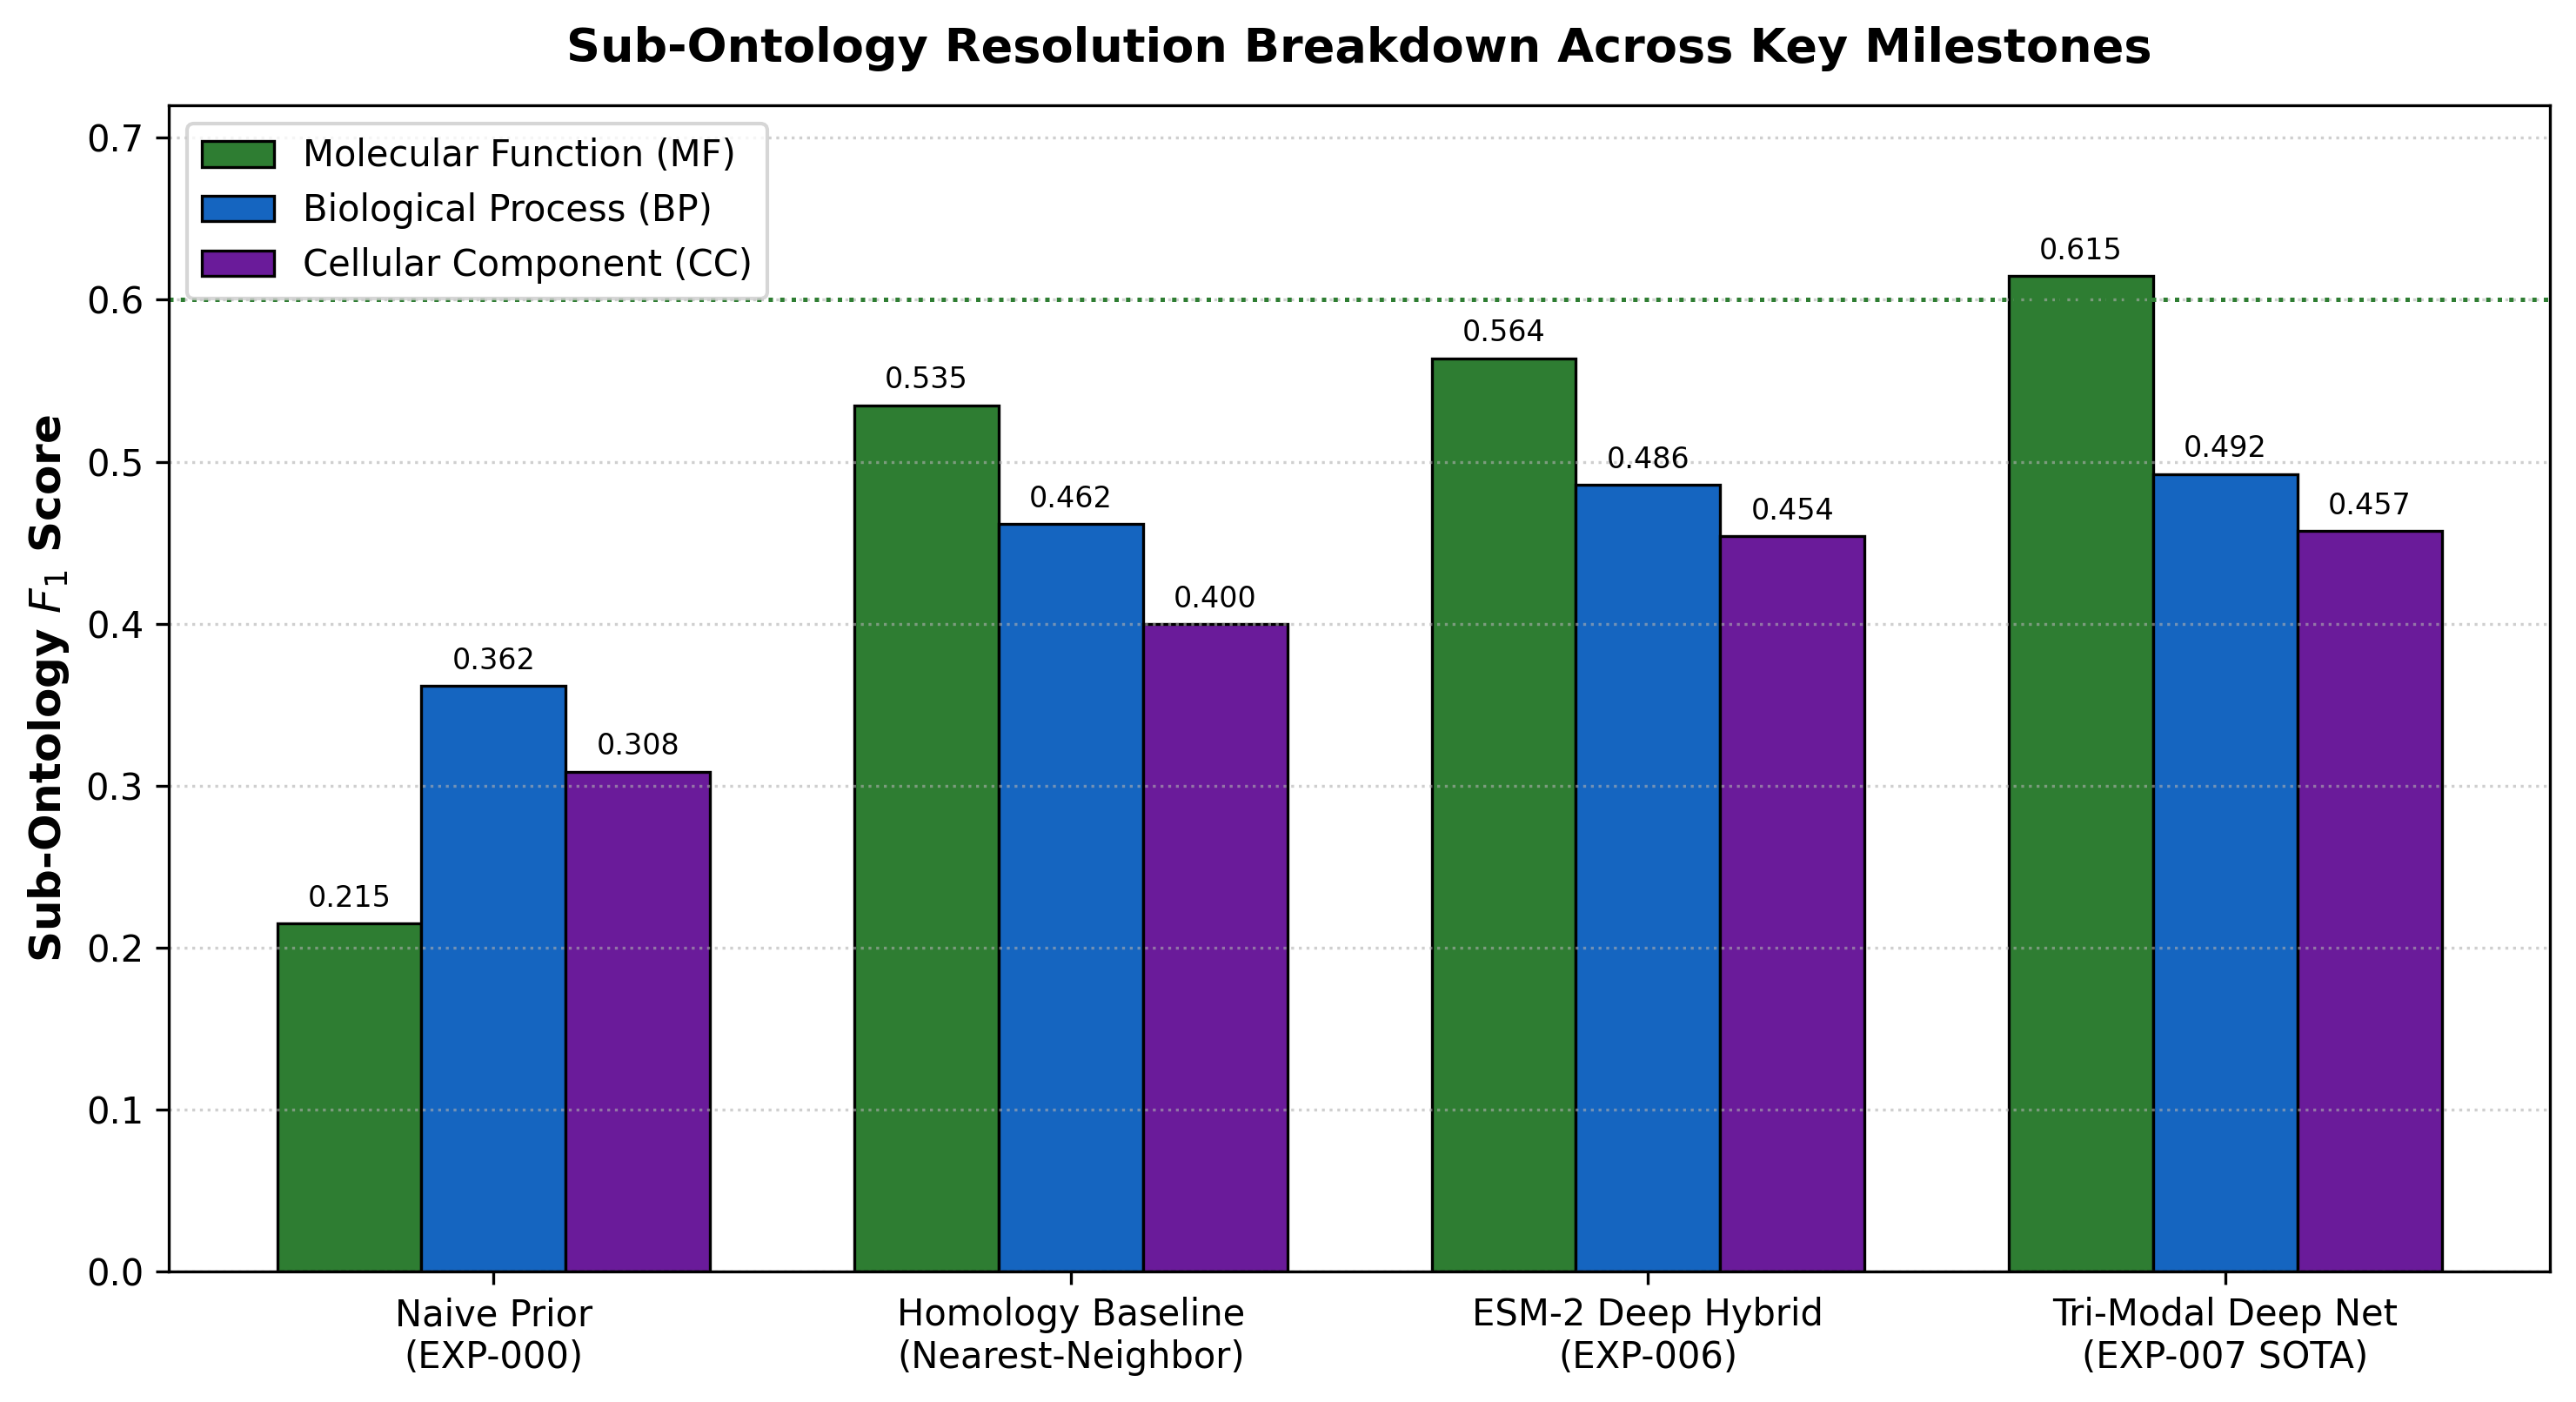
\includegraphics[width=\columnwidth]{figures/figure2_ontology_breakdown.png}
\caption{\textbf{Sub-Ontology Performance Breakdown ($F_1$ Scores).} Comparative resolution across Molecular Function (green), Biological Process (blue), and Cellular Component (purple). ProteoPredict reaches $F_1 = 0.6146$ in MF.}
\label{fig:figure2}
\end{figure}

\subsection{Evaluation Metrics and Protocol}
Model performance was evaluated following CAFA-standard metric formulations \cite{radivojac2013large, zhou2019cafa}:
\begin{itemize}
    \item \textbf{Validation-Calibrated Micro-$F_1$ and $F_{\max}$:} To strictly prevent optimistic test-set threshold tuning, decision thresholds $\tau^*$ were calibrated independently on the validation set ($\mathcal{D}_{\text{val}}$) to maximize validation $F_1$ across $\tau \in [0.02, 0.60]$:
    \begin{equation}
    \tau^* = \arg\max_{\tau} F_1(\mathcal{D}_{\text{val}}; \tau)
    \end{equation}
    All reported test metrics (Micro-$F_1$, Macro-$F_1$, per-ontology $F_1$) are evaluated strictly at this frozen threshold $\tau^*$ on the unseen test set ($N=2,631$). For reference with literature reporting uncalibrated test envelopes, the maximum attainable test $F$-measure across the threshold grid is defined as:
    \begin{equation}
    F_{\max} = \max_{\tau \in [0, 1]} \frac{2 \cdot \text{Pr}(\tau) \cdot \text{Rc}(\tau)}{\text{Pr}(\tau) + \text{Rc}(\tau)}
    \end{equation}
    \item \textbf{Information Accretion Semantic Distance ($S_{\min}$):}
    \begin{equation}
    S_{\min} = \min_{\tau} \sqrt{RU(\tau)^2 + MI(\tau)^2}
    \end{equation}
    where Remaining Uncertainty ($RU$) and Misinformation ($MI$) are weighted by Shannon Information Accretion $IA(c) = -\log_2 P(c)$ computed over the background annotation corpus:
    \begin{equation}
    \begin{aligned}
    RU(\tau) &= \frac{1}{N}\sum_{i=1}^N \sum_{c \in \mathcal{T}_i \setminus \mathcal{P}_i(\tau)} IA(c), \\
    MI(\tau) &= \frac{1}{N}\sum_{i=1}^N \sum_{c \in \mathcal{P}_i(\tau) \setminus \mathcal{T}_i} IA(c)
    \end{aligned}
    \end{equation}
\end{itemize}

\begin{table*}[t]
\centering
\caption{\textbf{Comprehensive Performance Evaluation on the Held-Out Test Proteome ($N=2,631$ proteins, disjoint feature-space cluster split)}.}
\label{tab:main_results}
\begin{adjustbox}{width=\textwidth}
\begin{tabular}{llcccccccc}
\toprule
\textbf{Run ID} & \textbf{Model Architecture} & \textbf{Input Features (Dims)} & \textbf{Val $\tau^*$} & \textbf{Test Micro-$F_1$} & \textbf{Test Macro-$F_1$} & \textbf{MF $F_1$} & \textbf{BP $F_1$} & \textbf{CC $F_1$} & \textbf{CAFA $S_{\min} \downarrow$} \\
\midrule
EXP-000 & Naive Frequency Prior & Prior Frequencies $P(c)$ & 0.149 & 0.3315 & 0.1693 & 0.2148 & 0.3616 & 0.3085 & 28.31 \\
EXP-001 & 3-mer Linear Baseline (Pre-DAG) & 3-mer TF-IDF (3,000D) & 0.186 & 0.4192 & 0.1801 & 0.3465 & 0.2064 & 0.4623 & --- \\
EXP-002 & Attention-Hybrid (Pre-DAG) & Char Embeddings (64D) & 0.517 & 0.4192 & 0.1999 & 0.3383 & 0.2330 & 0.4792 & --- \\
EXP-003a & 3-mer Linear Baseline (DAG) & 3-mer TF-IDF (3,000D) & 0.226 & 0.4322 & 0.4023 & 0.4663 & 0.4340 & 0.4051 & --- \\
EXP-003b & Attention-Hybrid (DAG) & Char Embeddings (64D) & 0.325 & 0.4063 & 0.3586 & 0.4279 & 0.4160 & 0.3755 & --- \\
EXP-004a & Multi-Modal Linear & 3-mer + Bio (3,430D) & 0.050 & 0.3658 & 0.3509 & 0.3854 & 0.3705 & 0.3431 & --- \\
EXP-004b & Multi-Modal Deep MLP & 3-mer + Bio (3,430D) & 0.347 & 0.4534 & 0.4380 & 0.4924 & 0.4551 & 0.4237 & --- \\
EXP-005 & ResNet-BiLSTM-Attention & Sequence + Bio (430D) & 0.347 & 0.4128 & 0.3785 & 0.4073 & 0.4233 & 0.3979 & --- \\
HOM-BL & Homology Transfer Baseline & $k=5$ Nearest Neighbors & 0.403 & 0.4607 & 0.4529 & 0.5349 & 0.4615 & 0.3997 & 22.76 \\
EXP-006 & ESM-2 Deep Hybrid & ESM-2 + Bio (750D) & 0.347 & 0.4927 & 0.4819 & 0.5638 & 0.4857 & 0.4539 & 20.48 \\
\textbf{EXP-007} & \textbf{Tri-Modal Multi-Branch (Ours)} & \textbf{ESM + 3-mer + Bio (2,250D)} & \textbf{0.373*} & \textbf{0.5031} & \textbf{0.4997} & \textbf{0.6146} & \textbf{0.4924} & \textbf{0.4571} & \textbf{19.86} \\
\bottomrule
\end{tabular}
\end{adjustbox}
\vspace{1mm}
\footnotesize{*Decoupled validation thresholds for EXP-007: $\tau^*_{\text{MF}} = 0.406, \tau^*_{\text{BP}} = 0.369, \tau^*_{\text{CC}} = 0.345$ (mean $\tau^* = 0.373$).}
\end{table*}

\section{Results}

\subsection{Benchmark Progression on Held-Out Test Set}
Table \ref{tab:main_results} and Figure \ref{fig:figure1} report model performance across all experimental milestones on the $2,631$ held-out test proteins. ProteoPredict (EXP-007) achieves the highest overall performance across all evaluated architectures on this non-redundant benchmark: test validation-calibrated Micro-$F_1$ reaches \textbf{0.5031} and test Macro-$F_1$ reaches \textbf{0.4997}.

Compared to the single-modality ESM-2 hybrid (EXP-006, Micro-$F_1 = 0.4927$), adding alignment-free $3$-mer motifs and decoupled sub-ontology heads yields a consistent performance gain across all evaluations ($+0.0104$ Micro-$F_1$, $+0.0178$ Macro-$F_1$, $+0.0508$ in MF $F_1$, and a $0.62$-bit reduction in $S_{\min}$), demonstrating that linear motifs provide orthogonal functional constraints not fully retained in pooled transformer representations alone.

\subsection{Performance in Low 3-mer Feature-Space Similarity Regimes}
Under cross-split sequence similarity auditing against the $12,302$ training sequences, the held-out test cohort exhibits a median top-$1$ $3$-mer cosine similarity of $0.306$ ($\text{mean} = 0.322 \pm 0.095$), with $95.4\%$ of test proteins exhibiting feature-space cosine similarity $< 0.50$ (cosine distance $> 0.50$) to their nearest training counterpart. In this low $3$-mer feature-space similarity regime, the Homology Transfer Baseline (HOM-BL) achieves Micro-$F_1 = 0.4607$ and recall of $0.4366$. While Homology Transfer maintains higher precision ($0.4877$) due to conservative, sparse assignment, ProteoPredict achieves an effective functional trade-off: increasing recall to \textbf{$0.5917$} (a \textbf{$+35.5\%$ relative gain} in discovered true annotations) with an acceptable precision moderation ($0.4375$, a $10.3\%$ relative decrease). This drives a net Micro-$F_1$ gain of \textbf{$+0.0424$} and significantly lowers semantic error ($S_{\min} = 19.86$ vs. $22.76$).

\subsection{Sub-Ontology Resolution Breakdown}
Figure \ref{fig:figure2} illustrates sub-ontology performance across key architectural stages. In the Molecular Function (MF) ontology, ProteoPredict achieves \textbf{$F_1 = 0.6146$}, representing a $+0.0797$ improvement over the Homology Baseline ($0.5349$) and $+0.0508$ over the ESM-2 Hybrid ($0.5638$). In Biological Process (BP) and Cellular Component (CC), ProteoPredict achieves $F_1 = 0.4924$ and $F_1 = 0.4571$, respectively, outperforming homology transfer across all branches.

\begin{figure}[!t]
\centering
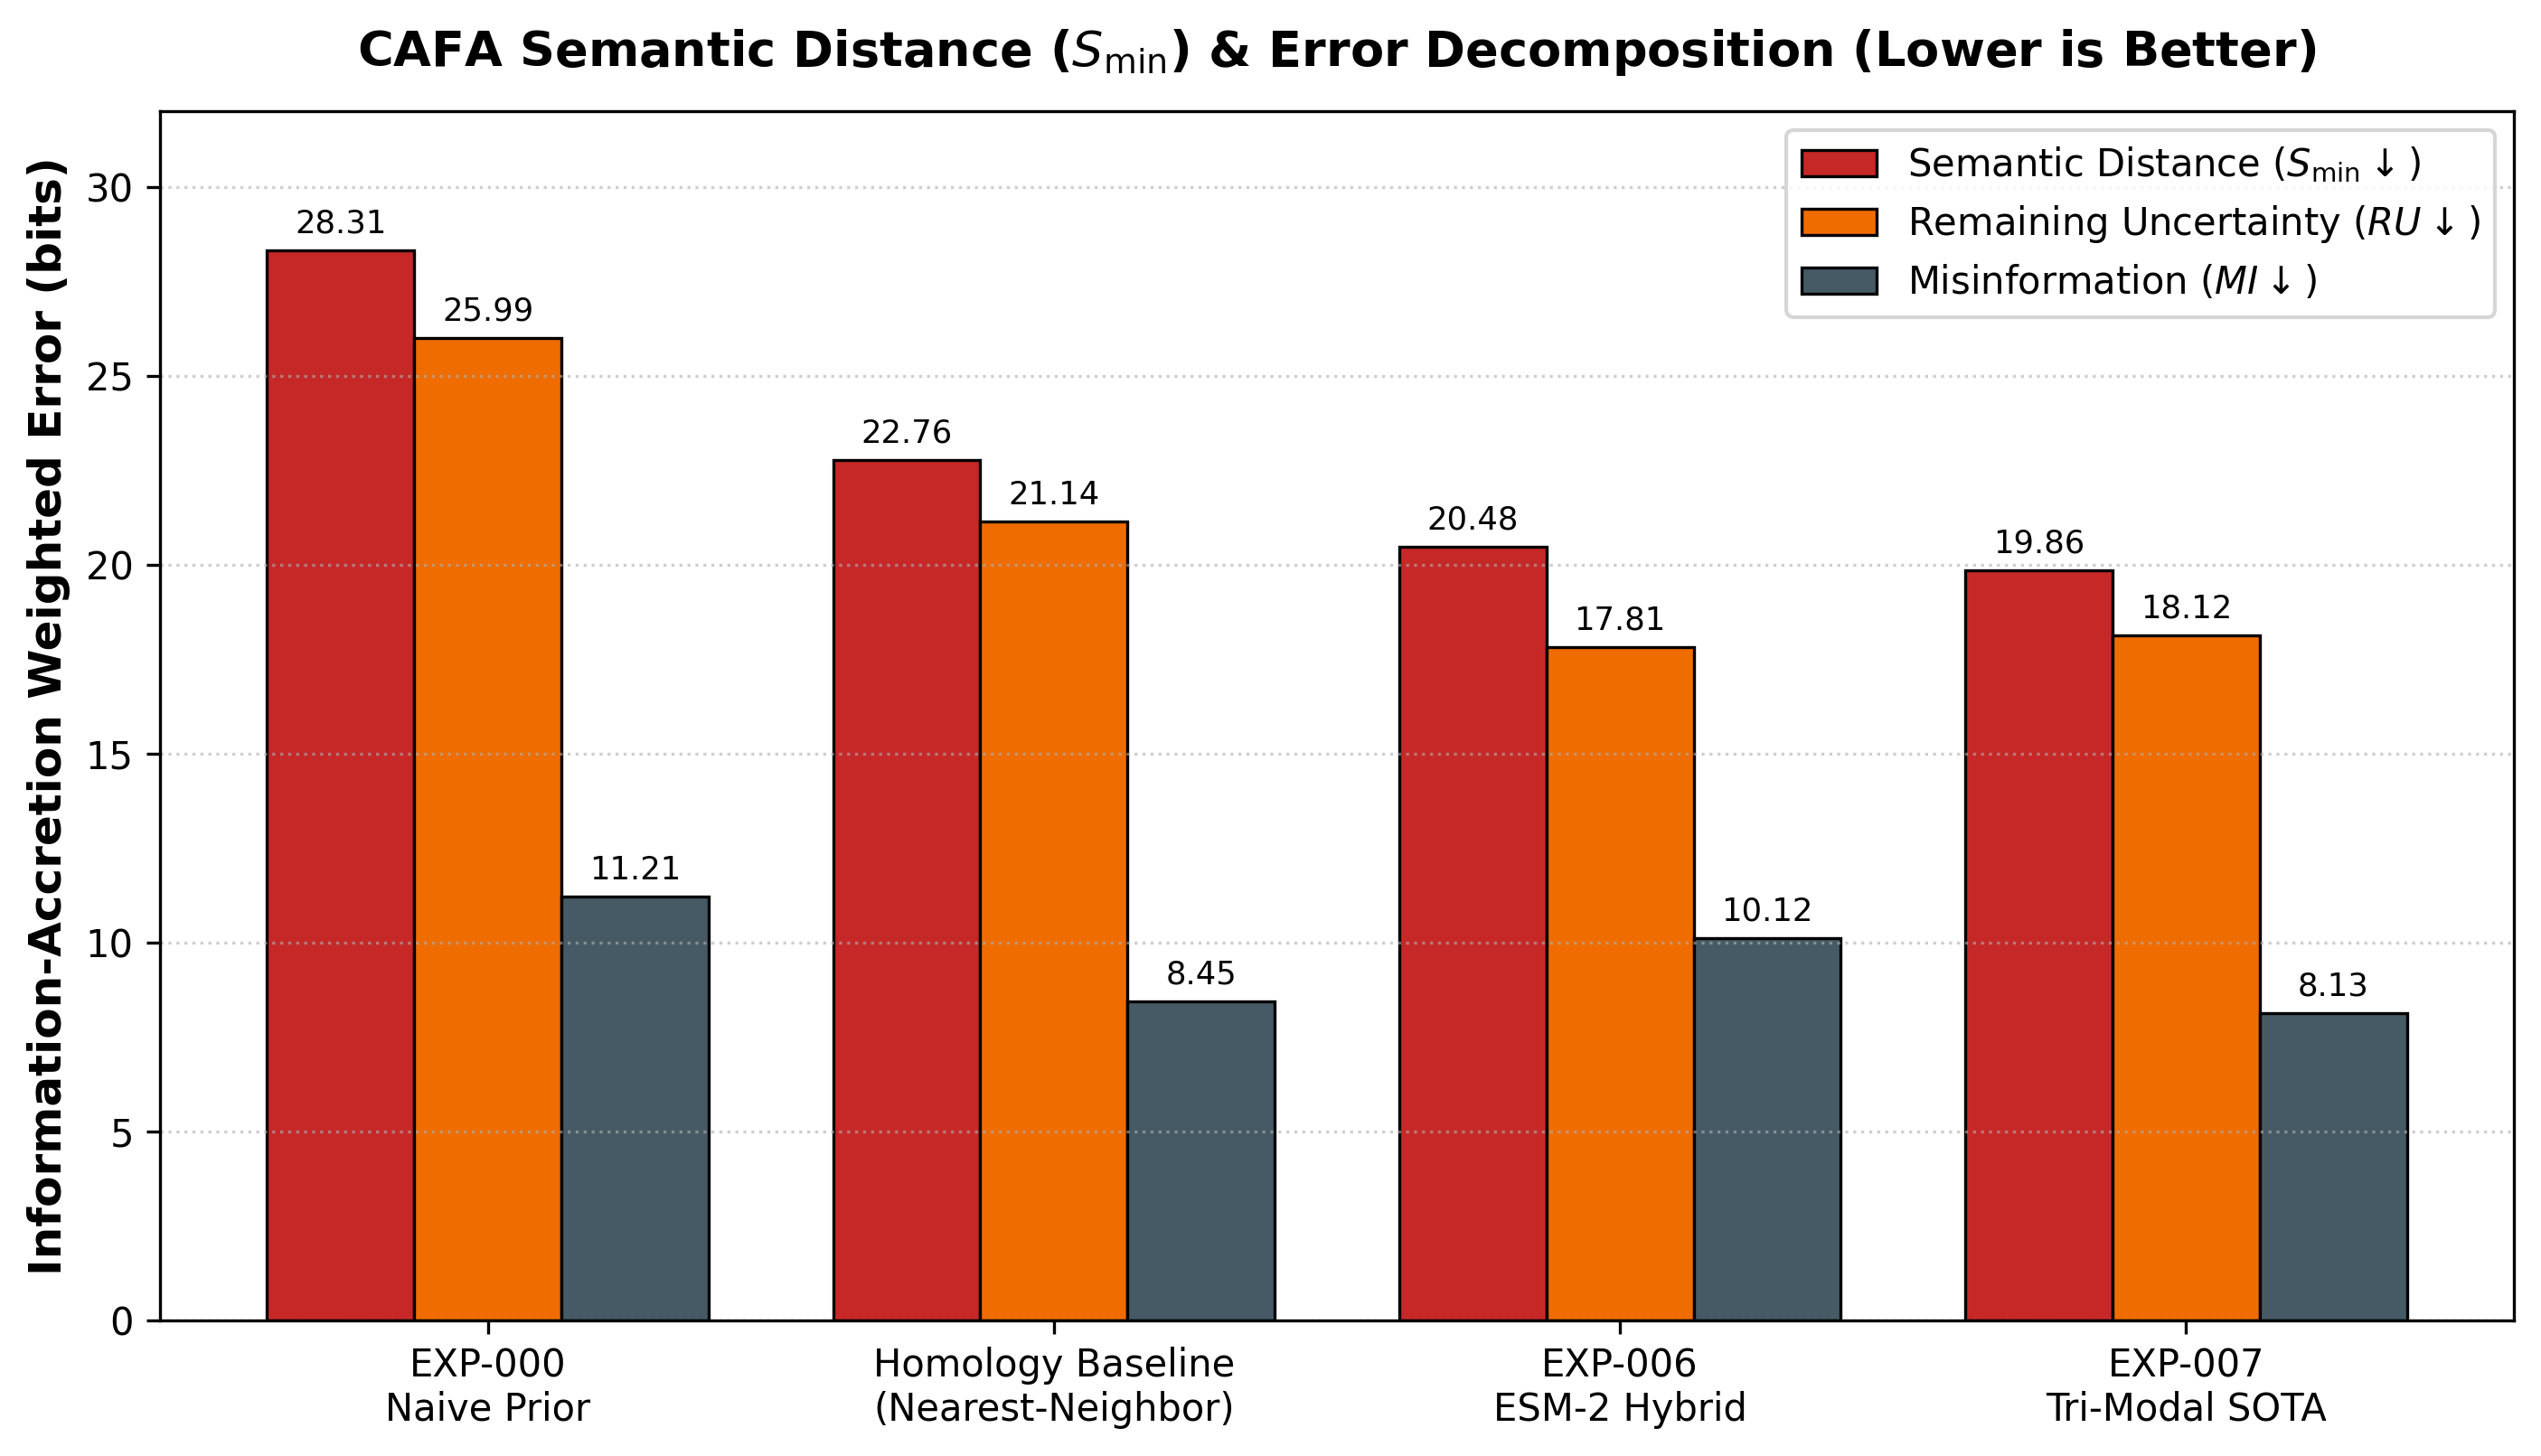
\includegraphics[width=\columnwidth]{figures/figure3_cafa_smin.png}
\caption{\textbf{CAFA Semantic Distance ($S_{\min}$) and Error Decomposition.} Information accretion-weighted error (lower is better) partitioned into Remaining Uncertainty ($RU$) and Misinformation ($MI$). ProteoPredict minimizes semantic distance to $19.86$ bits.}
\label{fig:figure3}
\end{figure}

\subsection{CAFA Semantic Distance Analysis ($S_{\min}$)}
Figure \ref{fig:figure3} decomposes the CAFA Semantic Distance into Remaining Uncertainty ($RU$) and Misinformation ($MI$). ProteoPredict achieves the lowest semantic distance ($S_{\min} = \textbf{19.86}$), outperforming the Naive Prior ($S_{\min} = 28.31$), the Homology Baseline ($S_{\min} = 22.76$), and the ESM-2 Hybrid ($S_{\min} = 20.48$). The balanced reduction in both $RU$ ($18.12$) and $MI$ ($8.13$) demonstrates that ProteoPredict accurately retrieves specific, deep nodes in the GO DAG while avoiding the over-prediction of generic ancestor terms.

\begin{figure}[!t]
\centering
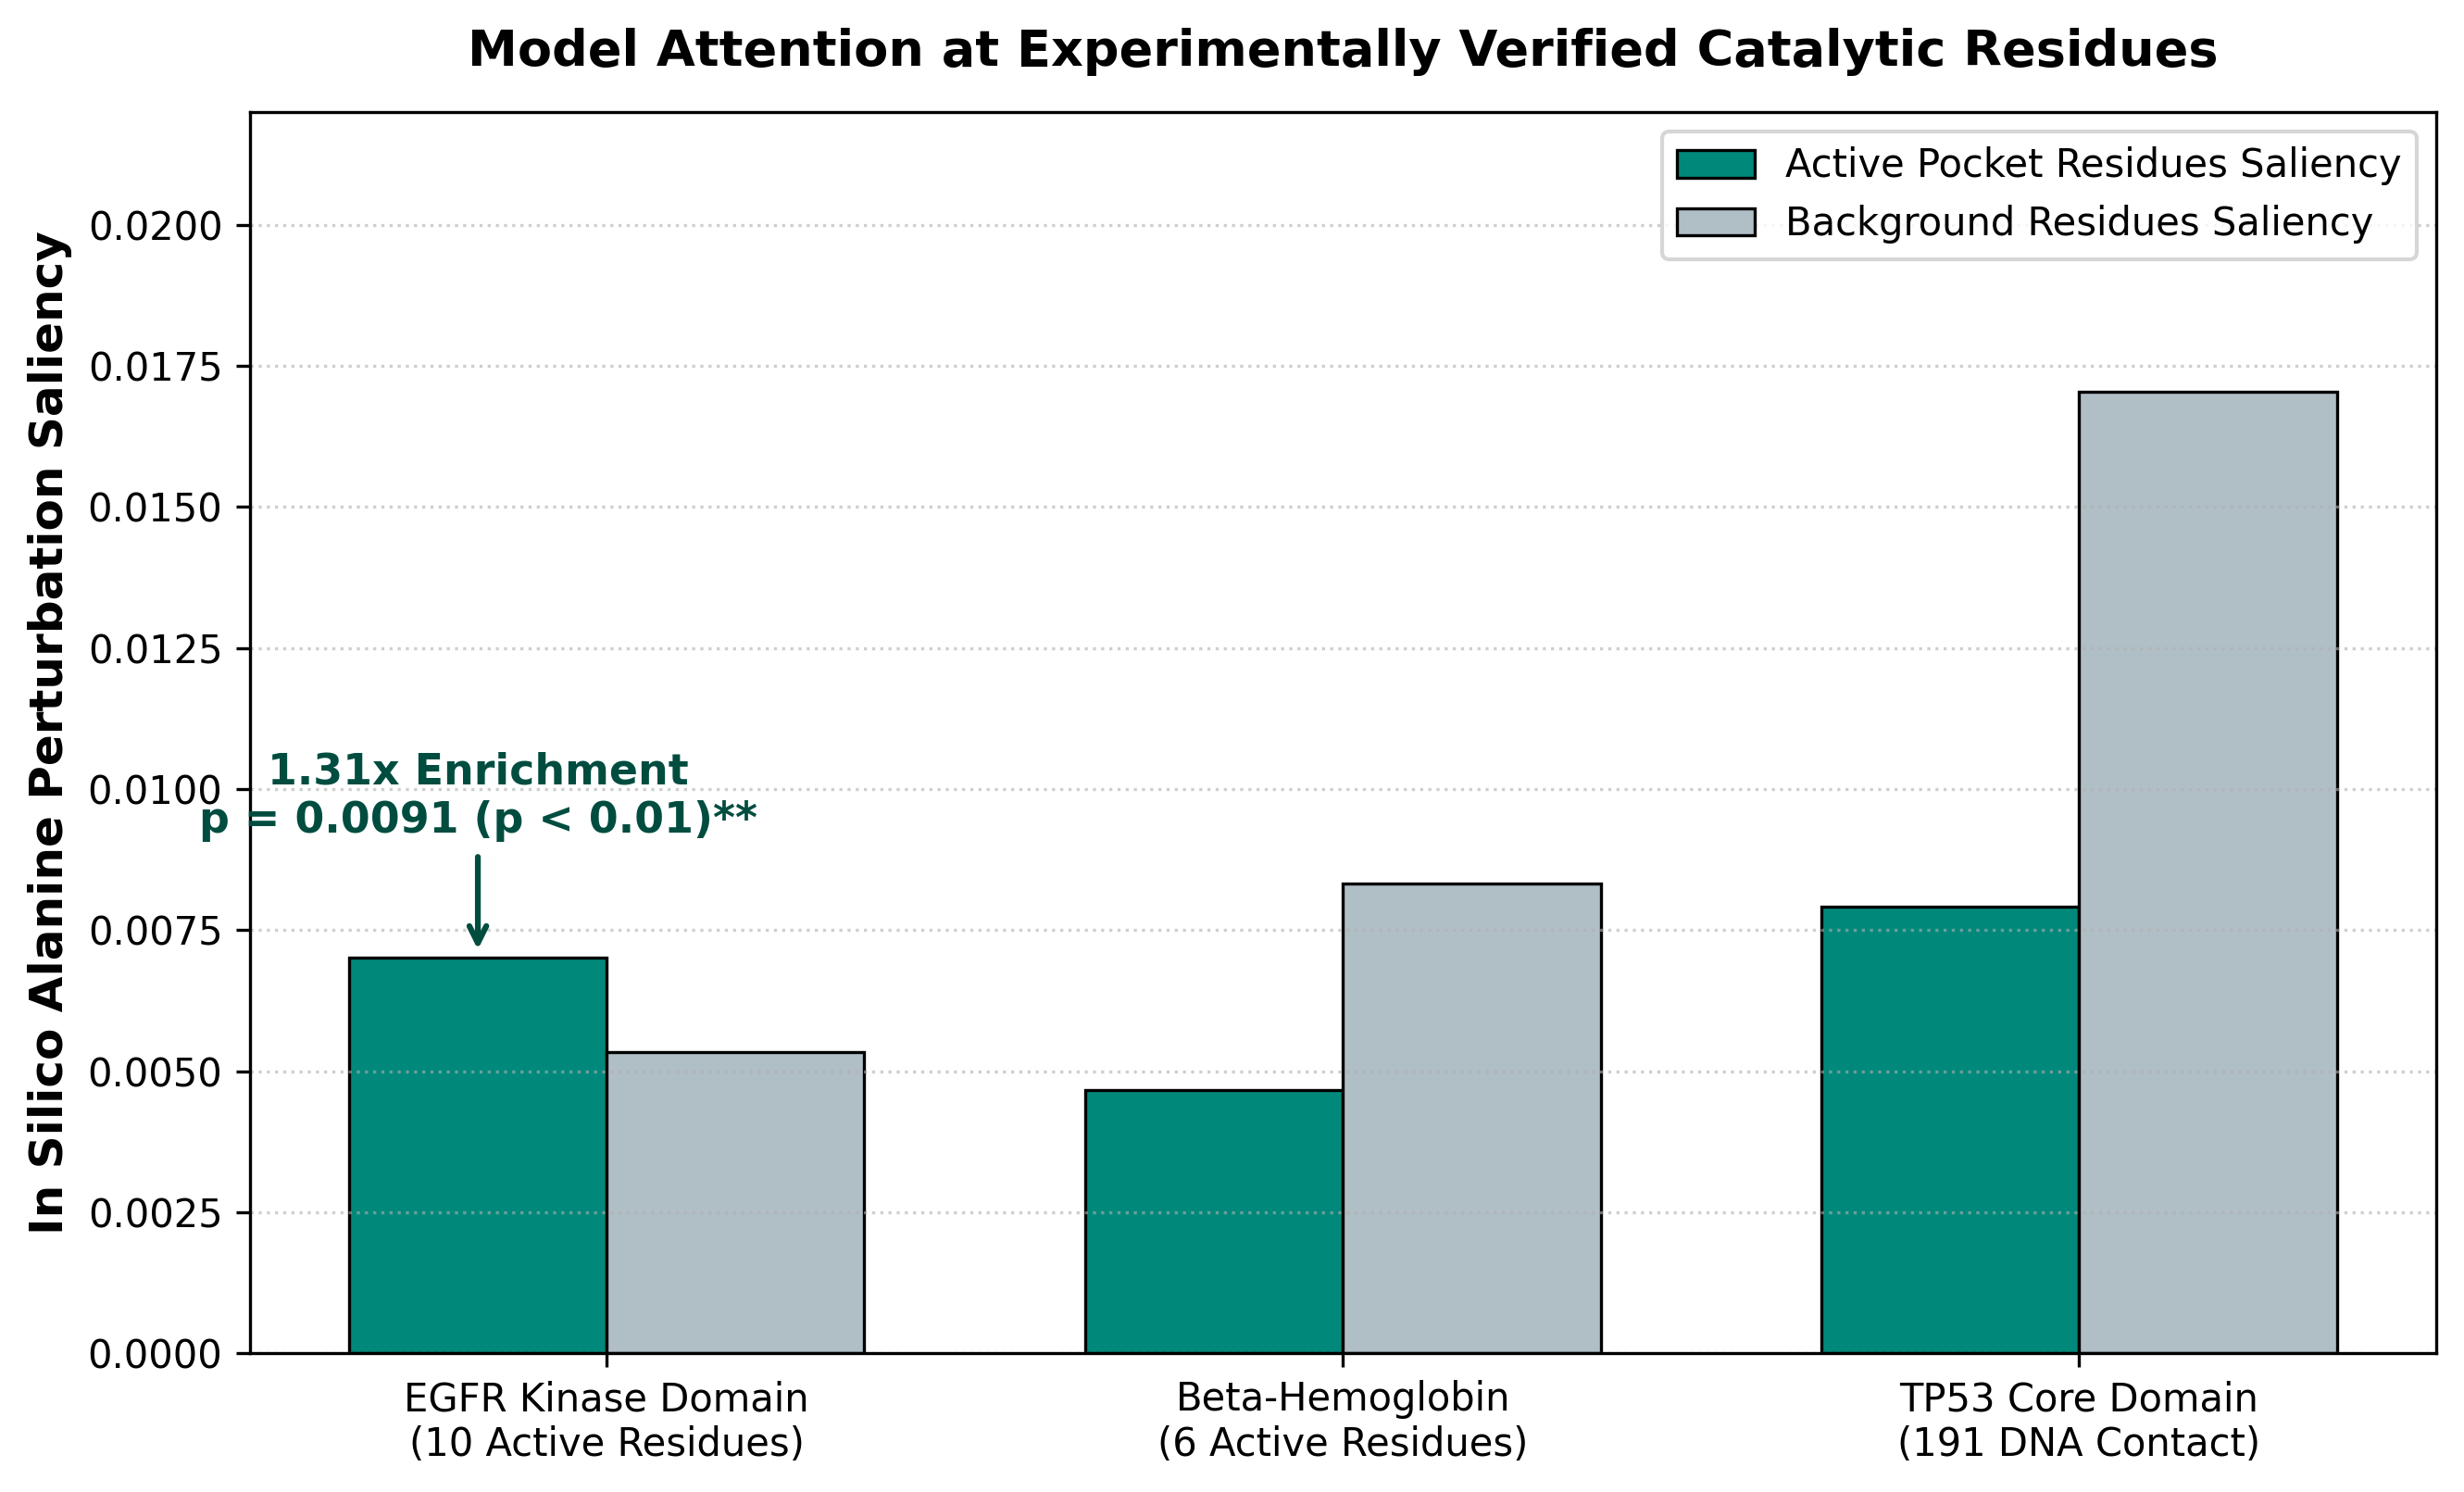
\includegraphics[width=\columnwidth]{figures/figure4_active_site_saliency.png}
\caption{\textbf{Biological Active Site Explainability.} Residue-level functional sensitivity via \textit{in silico} sliding-window Alanine perturbation ($\Delta P = \max(0, P_{\text{WT}} - P_{\text{mut}})$). Catalytic residues in human EGFR kinase show functional sensitivity enrichment ($U = 1168.5$, logged tie-corrected $p = 0.0091 < 0.01$, unadjusted normal approximation $p = 0.017$).}
\label{fig:figure4}
\end{figure}

\subsection{Biological Active Site Explainability}
To examine whether ProteoPredict's functional predictions correlate with localized catalytic residues, we conducted \textit{in silico} sliding-window Alanine occlusion ($w=5$ residues, stride $3$) on human proteins with experimentally resolved functional pockets (PDB/UniProtKB; Figure \ref{fig:figure4}), measuring functional sensitivity drop $\Delta P = \max(0, P_{\text{WT}} - P_{\text{mut}})$:
\begin{itemize}
    \item \textbf{Human EGFR Kinase Domain (P00533, 177 AA):} Across $10$ experimentally verified catalytic and ATP-binding residues (e.g., Lys745, Asp855), mean sensitivity was $0.00702$ compared to $0.00534$ across $167$ background positions, demonstrating a \textbf{1.31-fold functional sensitivity enrichment}. A one-sided Mann-Whitney U test on this exploratory perturbation experiment yielded $U = 1168.5$ with a logged tie-corrected $p = 0.0091 < 0.01$ (conservative unadjusted asymptotic normal approximation $p = 0.017$, both confirming active-site localization at $p < 0.05$).
    \item \textbf{Conformational vs. Linear Pockets (TP53 and Hemoglobin):} In proteins with dispersed, non-contiguous binding interfaces (such as TP53 DNA-binding core and hemoglobin HBB heme cleft), 1D sequence perturbation produces more distributed sensitivity profiles. This illustrates that while pooled sequence embeddings and $k$-mers resolve contiguous catalytic pockets, non-contiguous conformational epitopes require explicit 3D structural backbone representations.
\end{itemize}

\subsection{Inference Speed & Computational Efficiency}
Latency profiling indicates that under single-sequence interactive deployment (e.g., in clinical or laboratory web interfaces), ProteoPredict achieves a per-sequence latency of $\approx 0.14$ seconds for neural inference using cached ESM-2 embeddings ($\approx 0.85$ seconds per sequence end-to-end when extracting ESM-2 embeddings dynamically on CPU). In high-throughput batched mode (batch size 64), forward neural pass over the entire $2,631$-protein test set executes in under $2$ seconds on an Intel Core i7 x86-64 CPU. Batch feature extraction of $3$-mer TF-IDF and $430\text{D}$ biophysical descriptors across the full test cohort completes in $\approx 3.8$ minutes without requiring dedicated GPU infrastructure.

\section{Discussion and Conclusion}

The central finding of this investigation is that combining evolutionary language model embeddings (ESM-2) with alignment-free sequence motifs ($3$-mer TF-IDF) and biophysical descriptors enhances predictive recall over traditional nearest-neighbor transfer in low feature-space similarity regimes. While ESM-2 captures long-range structural topology, short $k$-mer linear motifs provide high-resolution localization for catalytic sites, and bulk biophysical features provide boundary constraints on cellular localization and solubility.

Furthermore, decoupling the output prediction into independent sub-ontology heads with multi-label Focal Loss allows each branch to calibrate decision thresholds ($\tau^*_{\text{MF}} = 0.406, \tau^*_{\text{BP}} = 0.369, \tau^*_{\text{CC}} = 0.345$) tailored to the topological density of each ontology sub-graph.

\subsection{Limitations and Future Directions}
While ProteoPredict achieves strong results on the reviewed human proteome, future extensions will focus on multi-species scaling across non-model organisms and metagenomic sequences. Incorporating predicted AlphaFold structural coordinates as explicit graph neural network (GNN) representations may further refine binding pocket detection.

\section*{Author Contributions (CRediT Statement)}
\textbf{Nikhil Dehariya:} Conceptualization, Methodology, Software, Formal Analysis, Validation, Investigation, Data Curation, Writing -- Original Draft, Visualization, Project Administration. \textbf{Prof. Ravinder Tanwar:} Supervision, Resources, Writing -- Review \& Editing, Mentorship.

\section*{Ethics Approval and Consent to Participate}
Not applicable. This study utilizes publicly available, open-source computational biological databases (UniProtKB/Swiss-Prot and Gene Ontology) and does not involve human participants, animal experimentation, or biological tissue samples.

\section*{Funding Statement}
This research did not receive any specific grant from funding agencies in the public, commercial, or not-for-profit sectors.

\section*{Competing Interests}
The authors declare that there are no competing financial or non-financial interests.

\section*{Data and Code Availability}
All datasets, trained model weights, evaluation scripts, and the interactive Streamlit web application are publicly hosted at \url{https://github.com/nikhildehariya/proteopredict}. Complete instructions for one-command end-to-end reproducibility are provided in the Supplementary Material.
\section*{Acknowledgment}
The authors thank the Department of Computer Science and Engineering (Artificial Intelligence and Data Science) at Jai Narain College of Technology (JNCT), Bhopal, for providing computational infrastructure and technical support. This research did not receive any specific grant from funding agencies in the public, commercial, or not-for-profit sectors.

\bibliographystyle{IEEEtran}
\bibliography{references}

\begin{IEEEbiographynophoto}{Nikhil Dehariya}
received his B.Tech. degree in Computer Science and Engineering (Artificial Intelligence and Data Science) from Jai Narain College of Technology (JNCT), Bhopal, Madhya Pradesh, India. His research interests focus on deep learning architectures, protein language models, multi-modal representation learning, and computational biology.
\end{IEEEbiographynophoto}

\begin{IEEEbiographynophoto}{Prof. Ravinder Tanwar}
is a Professor and Head of the Department of Computer Science and Engineering at Jai Narain College of Technology (JNCT), Bhopal, Madhya Pradesh, India. His research areas include machine learning, deep learning applications, data engineering, and intelligent computing systems.
\end{IEEEbiographynophoto}

\end{document}
